% act_1.5
\subsection{Joint PD control - critical damping}
The objective of this activity is display the UR5 robot on rviz and control the motion of its joints with a PD control law. The simulation starts with the initial joint configuration $\begin{bmatrix} \pi & -\frac{\pi}{8} & -\frac{\pi}{6} & 0.0 & 0.0 & 0.0 \end{bmatrix}$ and then move the second and fifth joint. On one hand, the two joints will maintain the initial configuration during the first $2$ seconds and follow a step reference during the last $3$ seconds. On the other hand, the two joints  will move with a sinusoidal reference during the first $4$ seconds and  maintain a constant joint position during the last second. The performance of the control method will be evaluated in next subsections.

\subsubsection{Step reference}
The Algorithm \ref{lst:joint_PD_control_critical_damping} move the second and fifth joints of the UR5 robot with a constant reference. Figure \ref{fig:act_1.5_joint_position}-\ref{fig:act_1.5_joint_acceleration} show the performance of the PD control method with $K_p=300$ $\mathrm{\frac{N.m}{rad}}$ and $K_{d,i}= 2 \sqrt{k_{p,i} m_{i,i}} $ $\mathrm{\frac{N.m.s}{rad}}$. The Figure \ref{fig:act_1.5_joint_position} shows the tracking performance of each joint of the UR5 robot. On one hand, the second joint ($\mathrm{q}_2$) does not present overshoot and steady state error close to $-0.18$ rad. On the other hand, the fifth joint ($\mathrm{q}_5$) does not present overshoot and steady state error close to $0$ rad. The variation of the temporal parameters of each joint is due to the control gains and the physical characteristics of the system. On one hand, the second joint must lift more mass than the fifth joint; and in the same way, the end effector of the robot is further from the second joint than from the fifth joint. On the other hand, the torque generated by the weight of the robot on the second joint can be calculated as $m g l \sin({\frac{\pi}{2} + \frac{\pi}{8}}) \approx -70$ N.m and the torque applied by the control method, at steady state, can be calculated as $K_p \theta_{\mathrm{error}}$, then equating both equations it is obtained that the error in steady state is $\approx -0.2$ rad. Finally, the Figure \ref{fig:act_1.5_k_d} show the variation of the derivative gain ($k_d$) of PD control method with critical damping approach and with a step reference. The new value of derivative gain of the second joint is $67.5$ $\mathrm{\frac{N.m.s}{rad}}$ and of the fifth joint is $17.5$ $\mathrm{\frac{N.m.s}{rad}}$. 

\begin{lstlisting}[language=Python,caption={Move the second and fifth joint of UR5 robot with the requirement motion of activity 1.5.1}, label={lst:joint_PD_control_critical_damping}]
# =========================
#   Configuration of node
# =========================
# create a node: 
rospy.init_node("node_joint_PD_control_critical_damping")

# public in topic /joint_states	to send joint data	
pub = rospy.Publisher('joint_states', JointState, queue_size=1000)

# loop rate (in Hz)
rate 	= rospy.Rate(1000)		# 100 [Hz]
dt 		= 1e-3					# 10  [ms]

# object(message) type JointState
jstate = JointState()

# ==========================================
#   Set initial joint configuration of UR5
# ==========================================
# initial configuration: position, velocity and acceleration 
q0 =   np.array([np.pi, -np.pi/8,  -np.pi/6, 0.0, 0.0, 0.0])
dq0 =  np.array([0.0, 0.0, 0.0, 0.0, 0.0, 0.0]) 
ddq0 = np.array([0.0, 0.0, 0.0, 0.0, 0.0, 0.0]) 

# desired trajectory: position, velocity and acceleration
q_des =   np.array([np.pi, -np.pi/8,  -np.pi/6, 0.0, 0.0, 0.0]) 
dq_des =  np.array([0.0, 0.0, 0.0, 0.0, 0.0, 0.0]) 
ddq_des = np.array([0.0, 0.0, 0.0, 0.0, 0.0, 0.0]) 

# measured trajectory: position, velocity and acceleration
q =   np.array([np.pi, -np.pi/8,  -np.pi/6, 0.0, 0.0, 0.0])
dq =  np.array([0.0, 0.0, 0.0, 0.0, 0.0, 0.0]) 
ddq = np.array([0.0, 0.0, 0.0, 0.0, 0.0, 0.0]) 

# ===========================
#   UR5 robot configuration
# ===========================
# joints name of UR5 robot
jnames = ['shoulder_pan_joint', 'shoulder_lift_joint', 'elbow_joint','wrist_1_joint', 'wrist_2_joint', 'wrist_3_joint']

# number of degress of freedom
ndof = 6
# the class robot load the ur5.urdf
ur5_robot = Robot(ndof,q0, dq0, dt)
# create inertia matrix 
M = np.zeros([ndof,ndof])
# create nonlinear effects vector
b = np.zeros(ndof)
# create gravity vector
g = np.zeros(ndof)

# ===============================
#   PD controller configuration
# ===============================
# proportional gain
kp = 300*np.ones(ndof)
# control vector
tau = np.zeros(ndof)    

#===============
#   Simulation
#===============
t = 0.0             # [sec] 
sim_duration = 5.0  # [sec]
step_start = 2.0    # [sec]

while not rospy.is_shutdown():
    # generate step reference after 2 seconds
    if t>=step_start:
        # second link
        q_des[1], dq_des[1], ddq_des[1] = step_reference_generator(q0[1], -0.4)
        # fifth link
        q_des[4], dq_des[4], ddq_des[4] = step_reference_generator(q0[4], 0.5)

    # error: position and velocity
    e 	=  q_des - q
    de 	=  dq_des - dq    

    # compute inertia matrix
    M = ur5_robot.get_M()

    # update value of kd with critical damping approach
    # equation: kd_{i,i} = M_{i,i}*2*sqrt(kd_{i,i})
    kd = 2*np.sqrt(np.multiply(kp, M.diagonal()))


    # proportional-derivative control method
    tau = np.multiply(kp, e) + np.multiply(kd, de)
    
    # send control signal
    ur5_robot.send_control_command(tau)
    # update states
    q, dq, ddq = ur5_robot.read_joint_position_velocity_acceleration()

    # publish message
    jstate.header.stamp = rospy.Time.now()
    jstate.name 		= jnames			# Joints position name
    jstate.position 	= q
    jstate.velocity 	= dq
    pub.publish(jstate)

    # update time
    t = t + dt

    if t>=sim_duration:
        # stop simulation
        print("stopping rviz ...")
        break
    rate.sleep()
\end{lstlisting}

\begin{figure}[H]
    \centering
    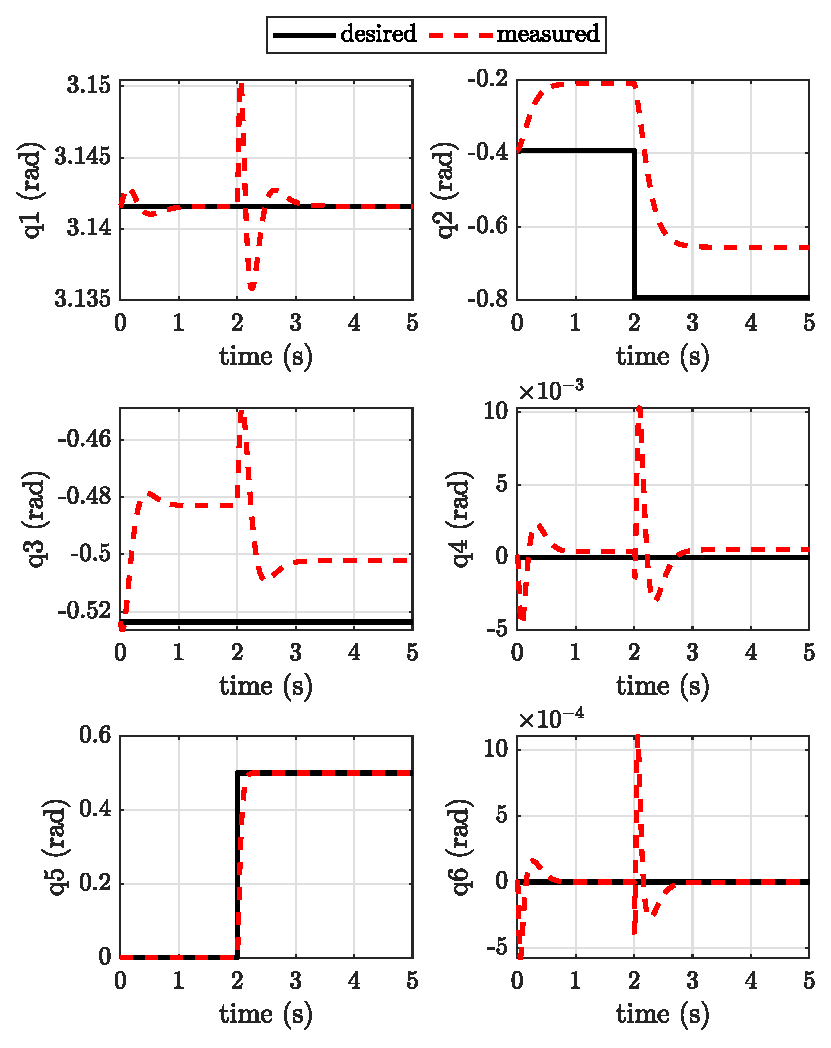
\includegraphics{images/act_1.5_step/joint_position.eps}
    \caption{Angular position of each joint of UR5 robot with Algorithm \ref{lst:joint_PD_control_critical_damping}.}
    \label{fig:act_1.5_joint_position}
\end{figure}

\begin{figure}[H]
    \centering
    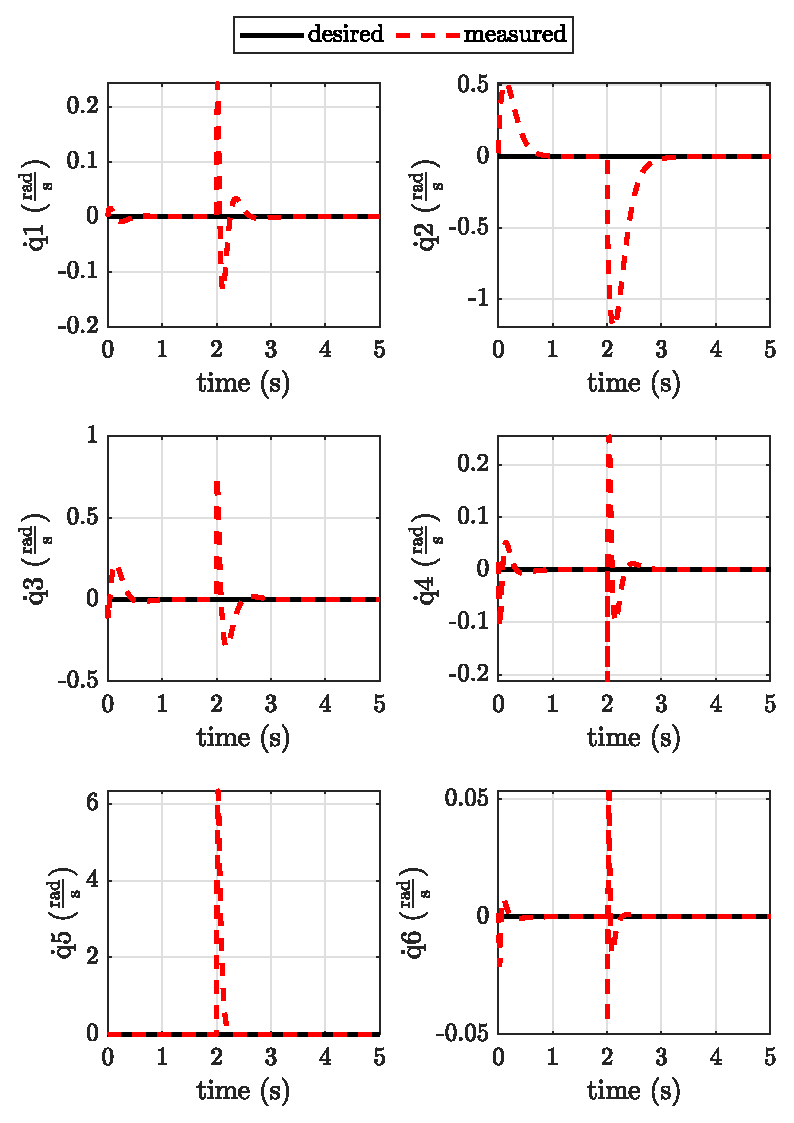
\includegraphics{images/act_1.5_step/joint_velocity.eps}
    \caption{Angular velocity of each joint of UR5 robot with Algorithm \ref{lst:joint_PD_control_critical_damping}.}
    \label{fig:act_1.5_joint_velocity}
\end{figure}

\begin{figure}[H]
    \centering
    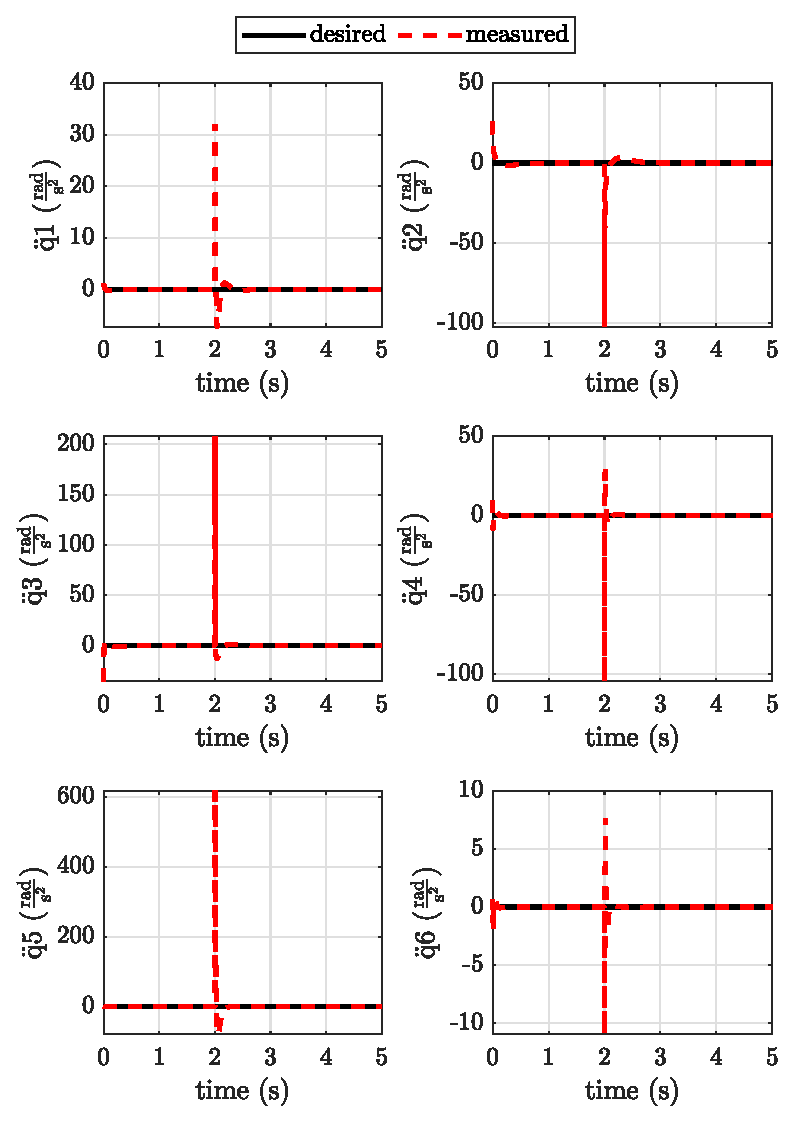
\includegraphics{images/act_1.5_step/joint_acceleration.eps}
    \caption{Angular acceleration of each joint of UR5 robot with Algorithm \ref{lst:joint_PD_control_critical_damping}.}
    \label{fig:act_1.5_joint_acceleration}
\end{figure}

\begin{figure}[H]
    \centering
    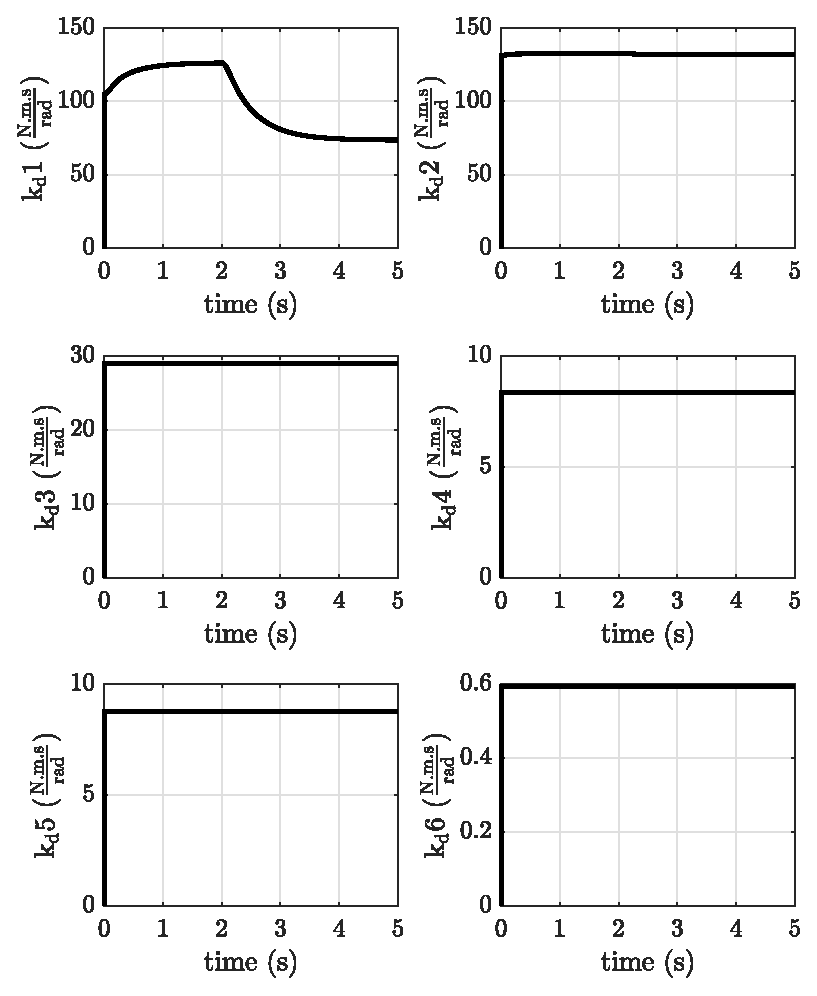
\includegraphics{images/act_1.5_step/kd.eps}
    \caption{The derivative gain ($k_d$) of the PD control method with critical damping formulation.}
    \label{fig:act_1.5_k_d}
\end{figure}



\newpage
\subsubsection{Sinusoidal reference}
The Algorithm \ref{lst:joint_PD_control_critical_damping_sinusoidal} move the second and fifth joints of the UR5 robot with a sinusoidal reference. Figure \ref{fig:act_1.5_sin_joint_position}-\ref{fig:act_1.5_sin_joint_acceleration} show the performance of the PD control method with $K_p=300$ $\mathrm{\frac{N.m}{rad}}$ and $K_{d,i}=2 \sqrt{k_{p,i}} m_{i,i}$ $\mathrm{\frac{N.m.s}{rad}}$. The Figure \ref{fig:act_1.5_sin_joint_position} shows the tracking performance of each joint of the UR5 robot. On one hand, the second joint ($\mathrm{q}_2$) does not present overshoot and steady state error close to $-0.14$ rad. On the other hand, the fifth joint ($\mathrm{q}_5$) does not present overshoot and steady state error close to $0$ rad. The variation of the temporal parameters of each joint is due to the control gains and the physical characteristics of the system. On one hand, the second joint must lift more mass than the fifth joint; and in the same way, the end effector of the robot is further from the second joint than from the fifth joint. On the other hand, the torque generated by the weight of the robot on the second joint can be calculated as $m g l \sin({\frac{\pi}{2} + \frac{\pi}{8}}) \approx -70$ N.m and the torque applied by the control method, at steady state, can be calculated as $K_p \theta_{\mathrm{error}}$, then equating both equations it is obtained that the error in steady state is $\approx -0.2$ rad. Finally, the Figure \ref{fig:act_1.5_sin_k_d} show the variation of the derivative gain ($k_d$) of PD control method with critical damping approach and with a step reference. The new value of derivative gain of the second joint is $67.5$ $\mathrm{\frac{N.m.s}{rad}}$ with oscillations of $\pm$ $0.5$ $\mathrm{\frac{N.m.s}{rad}}$ and of the fifth joint is $17.5$ $\mathrm{\frac{N.m.s}{rad}}$.  

\begin{lstlisting}[language=Python,caption={Move the second and fifth joint of UR5 robot with the requirement motion of activity 1.5.2}, label={lst:joint_PD_control_critical_damping_sinusoidal}]
# =========================
#   Configuration of node
# =========================
# create a node: 
rospy.init_node("node_joint_PD_control_critical_damping")

# public in topic /joint_states	to send joint data	
pub = rospy.Publisher('joint_states', JointState, queue_size=1000)

# loop rate (in Hz)
rate 	= rospy.Rate(1000)		# 100 [Hz]
dt 		= 1e-3					# 10  [ms]

# object(message) type JointState
jstate = JointState()

# ==========================================
#   Set initial joint configuration of UR5
# ==========================================
# initial configuration: position, velocity and acceleration 
q0 =   np.array([np.pi, -np.pi/8,  -np.pi/6, 0.0, 0.0, 0.0])
dq0 =  np.array([0.0, 0.0, 0.0, 0.0, 0.0, 0.0]) 
ddq0 = np.array([0.0, 0.0, 0.0, 0.0, 0.0, 0.0]) 

# desired trajectory: position, velocity and acceleration
q_des =   np.array([np.pi, -np.pi/8,  -np.pi/6, 0.0, 0.0, 0.0]) 
dq_des =  np.array([0.0, 0.0, 0.0, 0.0, 0.0, 0.0]) 
ddq_des = np.array([0.0, 0.0, 0.0, 0.0, 0.0, 0.0]) 

# measured trajectory: position, velocity and acceleration
q =   np.array([np.pi, -np.pi/8,  -np.pi/6, 0.0, 0.0, 0.0])
dq =  np.array([0.0, 0.0, 0.0, 0.0, 0.0, 0.0]) 
ddq = np.array([0.0, 0.0, 0.0, 0.0, 0.0, 0.0]) 

# ===========================
#   UR5 robot configuration
# ===========================
# joints name of UR5 robot
jnames = ['shoulder_pan_joint', 'shoulder_lift_joint', 'elbow_joint','wrist_1_joint', 'wrist_2_joint', 'wrist_3_joint']

# number of degress of freedom
ndof = 6
# the class robot load the ur5.urdf
ur5_robot = Robot(ndof,q0, dq0, dt)
# create inertia matrix 
M = np.zeros([ndof,ndof])
# create nonlinear effects vector
b = np.zeros(ndof)
# create gravity vector
g = np.zeros(ndof)

# ===============================
#   PD controller configuration
# ===============================
# proportional gain
kp = 300*np.ones(ndof)
# control vector
tau = np.zeros(ndof)    

#===============
#   Simulation
#===============
t = 0.0             # [sec] 
sim_duration = 5.0  # [sec]
sine_duration = 4.0 # [sec]

while not rospy.is_shutdown():
    # generate sinusoidal joint reference
    if t<=sine_duration:
        # second link
        q_des[1], dq_des[1], ddq_des[1] = sinusoidal_reference_generator(q0[1], dq0[1], ddq0[1], 0.2, 1, t)
        # fifth link
        q_des[4], dq_des[4], ddq_des[4] = sinusoidal_reference_generator(q0[4], dq0[4], ddq0[4], 0.4, 1.5, t) 

    # error: position and velocity
    e 	=  q_des - q
    de 	=  dq_des - dq    

    # compute inertia matrix
    M = ur5_robot.get_M()

    # update value of kd with critical damping approach
    # equation: kd_{i,i} = M_{i,i}*2*sqrt(kd_{i,i})
    kd = 2*np.sqrt(np.multiply(kp, M.diagonal()))

    # proportional-derivative control method
    tau = np.multiply(kp, e) + np.multiply(kd, de)
    
    # send control signal
    ur5_robot.send_control_command(tau)
    # update states
    q, dq, ddq = ur5_robot.read_joint_position_velocity_acceleration()

    # publish message
    jstate.header.stamp = rospy.Time.now()
    jstate.name 		= jnames			# Joints position name
    jstate.position 	= q
    jstate.velocity 	= dq
    pub.publish(jstate)

    # update time
    t = t + dt

    if t>=sim_duration:
        # stop simulation
        print("stopping rviz ...")
        break
    rate.sleep()
\end{lstlisting}


\begin{figure}[H]
    \centering
    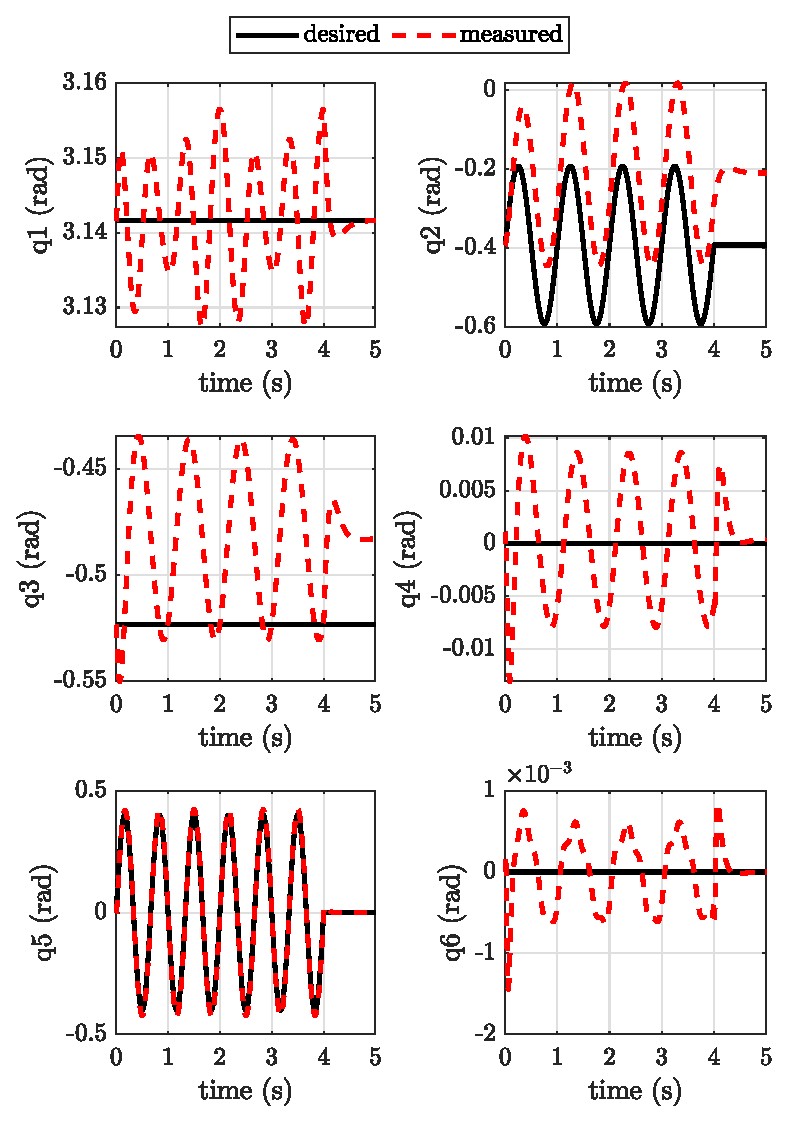
\includegraphics{images/act_1.5_sin/joint_position.eps}
    \caption{Angular position of each joint of UR5 robot with Algorithm \ref{lst:joint_PD_control_critical_damping_sinusoidal}.}
    \label{fig:act_1.5_sin_joint_position}
\end{figure}


\begin{figure}[H]
    \centering
    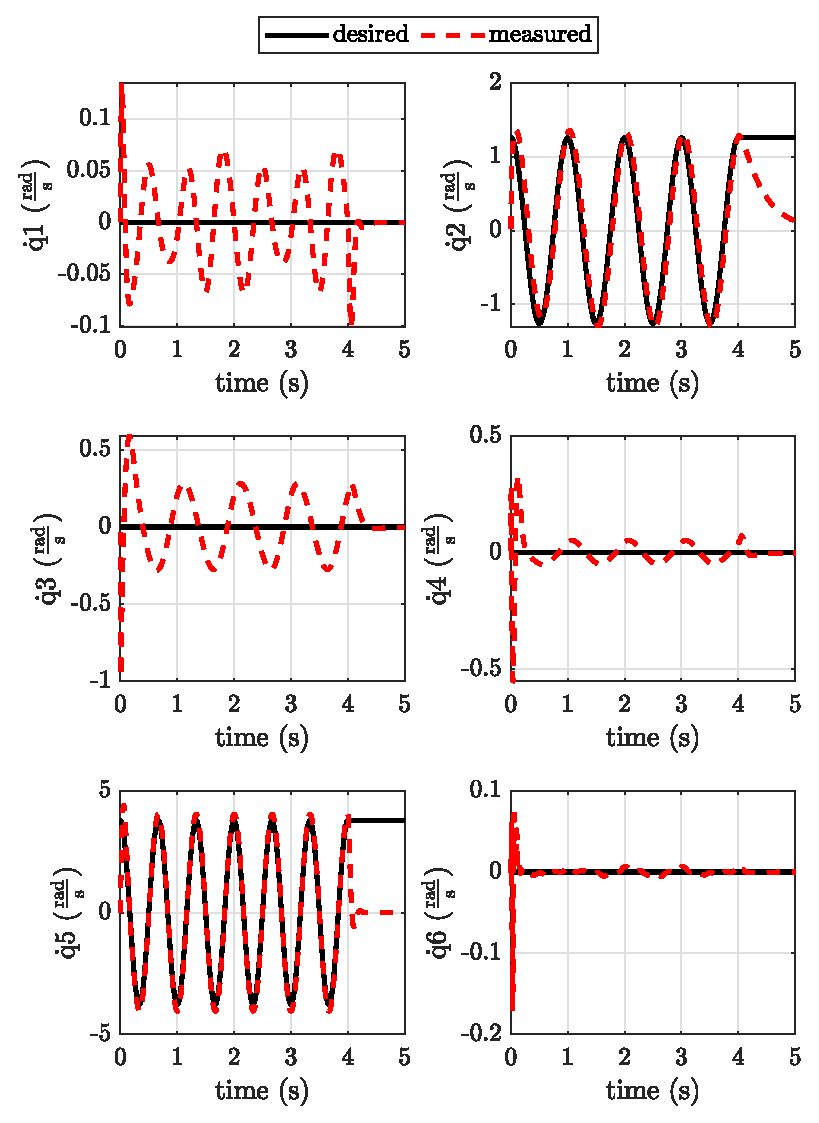
\includegraphics{images/act_1.5_sin/joint_velocity.eps}
    \caption{Angular velocity of each joint of UR5 robot with Algorithm \ref{lst:joint_PD_control_critical_damping_sinusoidal}.}
    \label{fig:act_1.5_sin_joint_velocity}
\end{figure}


\begin{figure}[H]
    \centering
    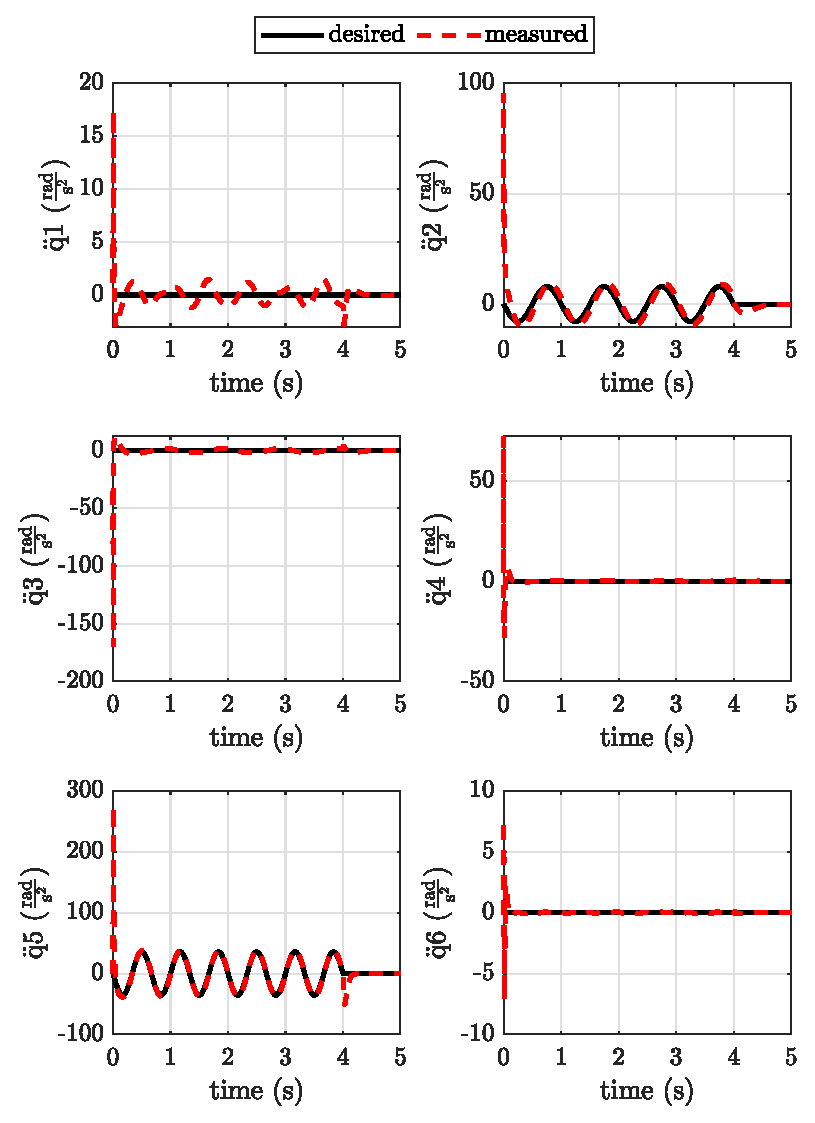
\includegraphics{images/act_1.5_sin/joint_acceleration.eps}
    \caption{Angular acceleration of each joint of UR5 robot with Algorithm \ref{lst:joint_PD_control_critical_damping_sinusoidal}.}
    \label{fig:act_1.5_sin_joint_acceleration}
\end{figure}


\begin{figure}[H]
    \centering
    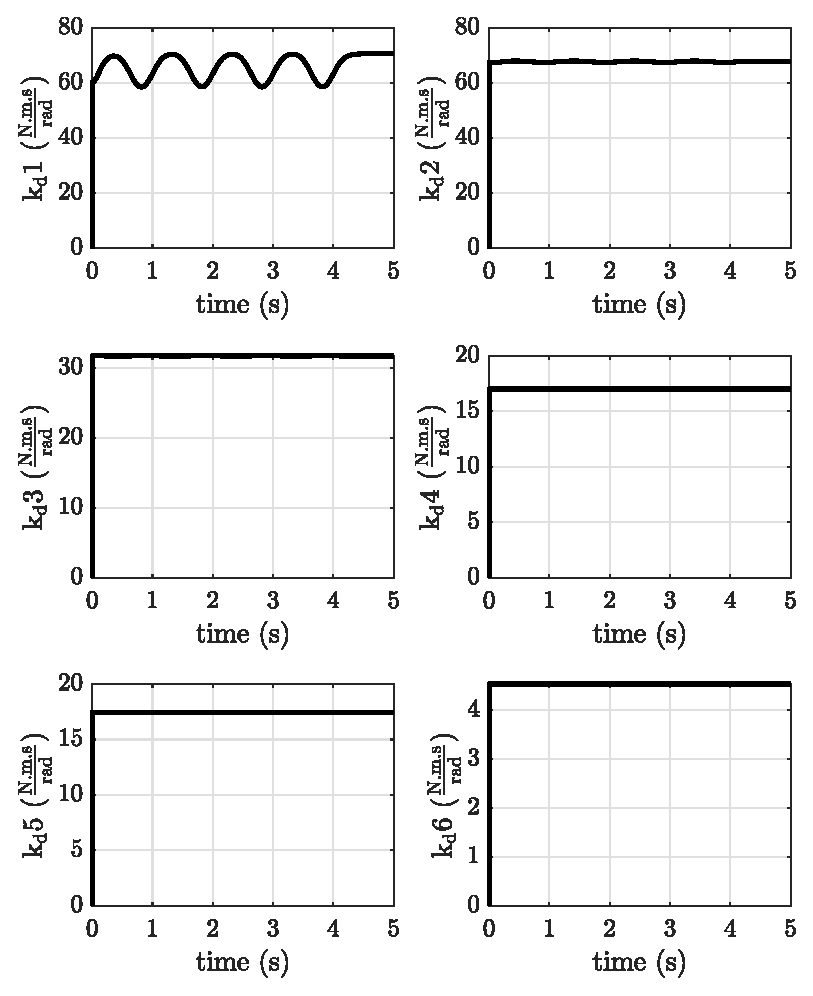
\includegraphics{images/act_1.5_sin/kd.eps}
    \caption{The derivative gain ($k_d$) of the PD control method with critical damping formulation.}
    \label{fig:act_1.5_sin_k_d}
\end{figure}